% This is text associated with the open textbook "Open Electromagnetics"
% See immediately below for author, date
% This work is licensed under the Creative Commons Attribution-ShareAlike 4.0 International License. (CC BY-SA 4.0) 
% To view a copy of the license, visit http://creativecommons.org/licenses/by-sa/4.0/

%ORB TITLE Radiation from a Hertzian Dipole
%ORB AUTHOR 0        # S.W. Ellingson, Virginia Tech (ellingson@vt.edu)
%ORB DATE 20191128   # yyyymmdd
%ORB ABSTRACT 

\label{m0197_Radiation_from_a_Hertzian_Dipole} % <-- Must match name of this file and module directory name.  Don't mess with this!
\index{Hertzian dipole|(}

Section~\ref{m0194_Radiation_Current_Moment} presented an informal derivation of the electromagnetic field radiated by a Hertzian dipole represented by a zero-length current moment.  
In this section, we provide a rigorous derivation using the concept of magnetic vector potential discussed in Sections~\ref{m0195_Magnetic_Vector_Potential} and \ref{m0196_Solution_of_the_Wave_Equation_for_Magnetic_Vector_Potential}. 
A review of those sections is recommended before tackling this section.

A Hertzian dipole is commonly defined as an electrically-short and infinitesimally-thin straight filament of current, in which the density of the current is uniform over its length.
The Hertzian dipole is commonly used as a ``building block'' for constructing physically-realizable distributions of current as exhibited by devices such as wire antennas. 
The method is to model these relatively complex distributions of current as the sum of Hertzian dipoles, which reduces the problem to that of summing the contributions of the individual Hertzian dipoles, with each Hertzian dipole having the appropriate (i.e., different) position, magnitude, and phase.

To facilitate use of the Hertzian dipole as a building block suitable for constructing physically-realizable distributions of current, we choose to represent the Hertzian dipole using an essentially equivalent current distribution which is mathematically more versatile.
This description of the Hertzian dipole replaces the notion of constant current over finite length with the notion of a \emph{current moment}
\index{current moment}
located at a single point. 
This is shown in Figure~\ref{m0197_fCurrentMoment},
%
\begin{figure}[b!] % <--- "[b!]" for first figure in section *only*; delete for 2nd and subsequent figures
\begin{center}
\pdftooltip{{  % note double braces
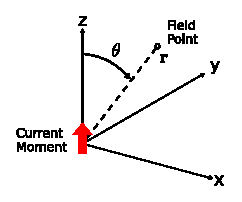
\includegraphics[width=2in]{modules/m0197_fCurrentMoment.eps} 
% https://commons.wikimedia.org/wiki/File:A_z-directed_current_moment_located_at_the_origin.svg
}}{An x-y-z Cartesian coordinate system with z vertical, x horizontal, and y into the page. For a field point labeled bold small r is an angle theta from the positive z axis. Thick arrow labeled “current moment” at the origin pointing up.}
\end{center}
\centerline{\scriptsize 
\copyright~\hyperref[m0197_fCurrentMoment_Credit]{C.\ Wang} 
\href{https://creativecommons.org/licenses/by-sa/4.0/}{CC BY-SA 4.0} 
} % \centerline  
\caption{
\label{m0197_fCurrentMoment}
A Hertzian dipole located at the origin, represented as a current moment. In this case, $\hat{\bf l}=\hat{\bf z}$.
}
\end{figure}
%
and is given by:
%
\begin{equation}
\Delta\widetilde{\bf J}({\bf r}) = \hat{\bf l}~\widetilde{I}~\Delta l~\delta({\bf r})
\end{equation}
%
where the product $\widetilde{I}\Delta l$ (SI base units of A$\cdot$m) is the current moment,
$\hat{\bf l}$ is the direction of current flow,
and $\delta({\bf r})$ is the volumetric sampling function defined as follows:
%
\begin{flalign}
~ &\delta({\bf r}) \triangleq 0~~~ \mbox{for}~~~ {\bf r}\neq 0;~~~ \mbox{and} \label{m0197_eDelta1} \\
~ &\int_{\mathcal{V}}\delta({\bf r})~dv \triangleq 1             \label{m0197_eDelta2}
\end{flalign}
%
where
$\mathcal{V}$ is any volume which includes the origin (${\bf r}=0$).
In this description, the Hertzian dipole is located at the origin. 

The solution for the magnetic vector potential due to a $\hat{\bf z}$-directed Hertzian dipole located at the origin was presented in Section~\ref{m0196_Solution_of_the_Wave_Equation_for_Magnetic_Vector_Potential}.  In the present scenario, it is:
%
\begin{equation}
\widetilde{\bf A}({\bf r}) = \hat{\bf z}~\mu~\widetilde{I}~\Delta l~\frac{e^{-\gamma r} }{4\pi r} 
\end{equation}
%
where the propagation constant $\gamma=\alpha+j\beta$ as usual.
Assuming lossless media ($\alpha=0$), we have
%
\begin{equation}
\widetilde{\bf A}({\bf r}) = \hat{\bf z}~\mu~\widetilde{I}~\Delta l~\frac{e^{-j\beta r} }{4\pi r} 
\end{equation}
%
We obtain the magnetic field intensity using the definition of magnetic vector potential:
%
\begin{flalign}
\widetilde{\bf H} &\triangleq (1/\mu)\nabla\times \widetilde{\bf A} \\
                  &= \frac{\widetilde{I}~\Delta l}{4\pi}~\nabla\times \hat{\bf z}~\frac{e^{-j\beta r} }{r} \label{m0197_H1} 
\end{flalign}
%
To proceed, it is useful to convert $\hat{\bf z}$ into the spherical coordinate system.  
To do this, we find the component of $\hat{\bf z}$ that is parallel to $\hat{\bf r}$, $\hat{\bf \theta}$, and $\hat{\bf \phi}$; and then sum the results:
%
\begin{flalign}
\hat{\bf z} 
&= \hat{\bf r}\left(\hat{\bf r}\cdot\hat{\bf z}\right)
  +\hat{\bf \theta}\left(\hat{\bf \theta}\cdot\hat{\bf z}\right)
  +\hat{\bf \phi}\left(\hat{\bf \phi}\cdot\hat{\bf z}\right) \\
&= \hat{\bf r}\cos\theta
  -\hat{\bf \theta}\sin\theta
  +0
\end{flalign}
%
Equation~\ref{m0197_H1}  requires computation of the following quantity:
%
\begin{flalign}
\nabla\times \hat{\bf z}\frac{e^{-j\beta r}}{r}  &= \nabla\times\left[ ~~~\hat{\bf r}     \left(\cos\theta\right)\frac{e^{-j\beta r}}{r} \right. \nonumber \\
                                                               &  ~~~~~~~~~~~~~~~  \left. -\hat{\bf \theta}\left(\sin\theta\right)\frac{e^{-j\beta r}}{r} \right] \label{m0197_e2}
\end{flalign}
%
At this point, it is convenient to make the following definitions:
%
\begin{flalign}
C_r        &\triangleq \left(\cos\theta\right)\frac{e^{-j\beta r}}{r} \\
C_{\theta} &\triangleq -\left(\sin\theta\right)\frac{e^{-j\beta r}}{r}
\end{flalign}
%
These definitions allow Equation~\ref{m0197_e2} to be written compactly as follows:
%
\begin{equation}
\nabla\times \hat{\bf z}\frac{e^{-j\beta r}}{r} = \nabla\times\left[ ~\hat{\bf r}C_r + \hat{\bf \theta}C_{\theta} \right] \label{m0197_e1}
\end{equation}
%
The right side of Equation~\ref{m0197_e1} is evaluated using Equation~\ref{m0139_eCurlSph} (Appendix~\ref{m0139_Vector_Operators}).
Although the complete expression consists of 6 terms, only 2 terms are non-zero.\footnote{Specifically, 
two terms are zero because there is no $\hat{\bf \phi}$ component in the argument of the curl function; and another two terms are zero because the argument of the curl function is independent of $\phi$, so partial derivatives with respect to $\phi$ are zero.}
This leaves:
%
\begin{flalign}
\nabla\times \hat{\bf z}\frac{e^{-j\beta r}}{r}  
  &= \hat{\bf \phi} \frac{1}{r} \left[ \frac{\partial}{\partial r}\left(r C_{\theta}\right) - \frac{\partial}{\partial \theta}C_r \right] \\
  &= \hat{\bf \phi} \left(\sin\theta\right) \frac{e^{-j\beta r}}{r} \left( j\beta + \frac{1}{r} \right)
\end{flalign}
%
Substituting this result into Equation~\ref{m0197_H1}, we obtain:
%
\begin{equation}
\widetilde{\bf H} = \hat{\bf \phi} \frac{\widetilde{I}~\Delta l}{4\pi}~\left(\sin\theta\right) \frac{e^{-j\beta r}}{r} \left( j\beta + \frac{1}{r} \right) \label{m0197_H2}
\end{equation}
%
Let us further limit our scope to the field far from the antenna.
Specifically, let us assume $r\gg\lambda$.
Now we use the relationship $\beta=2\pi/\lambda$ and determine the following:
%
\begin{flalign}
j\beta + \frac{1}{r} &= j\frac{2\pi}{\lambda} + \frac{1}{r} \\
                     &\approx j\frac{2\pi}{\lambda} =j\beta
\end{flalign}
Equation~\ref{m0197_H2} becomes:
%
\begin{equation}
\boxed{
\widetilde{\bf H} \approx \hat{\bf \phi} j \frac{\widetilde{I}\cdot\beta \Delta l}{4\pi}~\left(\sin\theta\right) \frac{e^{-j\beta r}}{r} \label{m0197_H4}
}
\end{equation}
%
where the approximation holds for low-loss media and $r\gg\lambda$.
This expression is known as a \emph{far field approximation}, 
\index{far field}
since it is valid only for distances ``far'' (relative to a wavelength) from the source.

Now let us take a moment to interpret this result:
\begin{itemize}
\item Notice the factor $\beta \Delta l$ has units of radians; that is, it is \emph{electrical length}.
\index{electrical length}
This tells us that the magnitude of the radiated field depends on the electrical length of the current moment.
\item The factor $e^{-j\beta r}/r$ indicates that this is a spherical wave; that is, surfaces of constant phase correspond to concentric spheres centered on the source, and magnitude is inversely proportional to distance.
\item The direction of the magnetic field vector is always $\hat{\bf \phi}$, which is precisely what we expect; for example, using the Biot-Savart law.
\index{Biot-Savart law}
\item Finally, note the factor $\sin\theta$.  This indicates that the field magnitude is zero along the direction in which the source current flows, and is a maximum in the plane perpendicular to this direction.
\end{itemize}

Now let us determine the electric field radiated by the Hertzian dipole.
The direct method is to employ Ampere's law.
\index{Ampere's law!general form}
That is,
%
\begin{equation}
\widetilde{\bf E} = \frac{1}{j\omega\epsilon} \nabla \times \widetilde{\bf H}
\end{equation}
%
where $\widetilde{\bf H}$ is given by Equation~\ref{m0197_H4}.
At field points far from the dipole, the radius of curvature of the spherical phasefronts is very large and so appear to be \emph{locally planar}. 
That is, from the perspective of an observer far from the dipole, the arriving wave appears to be a plane wave. 
In this case, we may employ the \emph{plane wave relationships}.
\index{plane wave relationships}
The appropriate relationship in this case is:
%
\begin{equation}
\widetilde{\bf E} = -\eta \hat{\bf r} \times \widetilde{\bf H}
\end{equation}
%
where $\eta$ is the wave impedance.
\index{wave impedance}
So we find:
%
\begin{equation}
\boxed{
\widetilde{\bf E} \approx \hat{\bf \theta} j\eta \frac{\widetilde{I}\cdot\beta \Delta l}{4\pi}~\left(\sin\theta\right) \frac{e^{-j\beta r}}{r} 
}
\label{m0197_eE}
\end{equation}
%
Summarizing:
%%%%%%%%%%%%%%%%%%%%%%%%%%%%%%%%%%%%%%%%%%%%%%%
%ORB HIGHLIGHT
\begin{mdframed}[backgroundcolor=yellow!20,nobreak=true] 
The electric and magnetic fields far (i.e., $\gg\lambda$) from a $\hat{\bf z}$-directed Hertzian dipole having constant current $\widetilde{I}$ over length $\Delta l$, located at the origin, are given by Equations~\ref{m0197_eE} and \ref{m0197_H4}, respectively. 
\end{mdframed}
%%%%%%%%%%%%%%%%%%%%%%%%%%%%%%%%%%%%%%%%%%%%%%%

%%%%%%%%%%%%%%%%%%%%%

{\bf Additional Reading:}
\begin{itemize}
\item ``\href{https://en.wikipedia.org/wiki/Dipole_antenna#Hertzian_dipole}{Dipole antenna}'' (section entitled ``Hertzian Dipole'') on Wikipedia.
\end{itemize}

\index{Hertzian dipole|)}


